\documentclass[lettersize,journal]{IEEEtran}
\usepackage{amsmath,amsfonts}
\usepackage{algorithmic}
\usepackage{algorithm}
\usepackage{array}
\usepackage[caption=false,font=normalsize,labelfont=sf,textfont=sf]{subfig}
\usepackage{textcomp}
\usepackage{stfloats}
\usepackage{url}
\usepackage{verbatim}
\usepackage{graphicx}
\usepackage{cite}
\hyphenation{op-tical net-works semi-conduc-tor IEEE-Xplore}
% updated with editorial comments 8/9/2021

\begin{document}

\title{Pengetahuan dan Kemampuan yang Dimiliki Pengguna Non-Ahli dalam Mendeteksi Phishing}

\author{IEEE Publication Technology,~\IEEEmembership{Adhi Wahyu Utama and Dimas Anwar Aziz,~Telkom University,}
  % <-this % stops a space
  \thanks{This paper was produced by the IEEE Publication Technology Group. They are in Piscataway, NJ.}% <-this % stops a space
  \thanks{Manuscript received April 19, 2021; revised August 16, 2021.}
}

% The paper headers
\markboth{Journal of \LaTeX\ Class Files,~Vol.~14, No.~8, August~2021}%
{Shell \MakeLowercase{\textit{et al.}}: A Sample Article Using IEEEtran.cls for IEEE Journals}

% \IEEEpubid{0000--0000/00\$00.00~\copyright~2021 IEEE}
% Remember, if you use this you must call \IEEEpubidadjcol in the second
% column for its text to clear the IEEEpubid mark.

\maketitle

\begin{abstract}
  Email phishing adalah komunikasi penipuan yang berpura-pura menjadi sesuatu yang bukan sebenarnya untuk membuat orang melakukan tindakan yang seharusnya tidak mereka lakukan. Kami melakukan survei terhadap beberapa orang dari berbagai demografi di Indonesia dan meminta mereka untuk berbagi pengalaman mereka terkait email phishing. Dari analisis pengalaman tersebut, kami menemukan bahwa cara pengguna email mendeteksi pesan phishing memiliki banyak kesamaan dengan cara ahli IT mengidentifikasi phishing. Kami juga menemukan bahwa pengguna email memiliki pengetahuan unik dan kemampuan berharga dalam proses identifikasi yang tidak dimiliki oleh kontrol teknis maupun ahli IT. Kami menyarankan bahwa pelatihan yang ditargetkan pada cara memanfaatkan keunikan ini kemungkinan akan meningkatkan pencegahan phishing.
\end{abstract}

\begin{IEEEkeywords}
  Phishing detection, non-expert users, email security, user capabilities, cybersecurity awareness, security training, user knowledge, online threats, digital literacy, human factors in security.
\end{IEEEkeywords}

\section{Introduction}
\IEEEPARstart{E}{mail} adalah salah satu metode komunikasi yang paling umum digunakan, terutama dalam organisasi besar dan e-commerce. Lebih dari 3,9 miliar orang memiliki akun email, dan secara kolektif mereka mengirim dan menerima lebih dari 290 miliar email per hari \cite{sebelas}. Email merupakan salah satu metode utama yang digunakan untuk berkomunikasi dengan orang asing. Namun, karena email adalah sistem global di mana siapa saja dapat berkomunikasi dengan siapa saja, pelaku kejahatan mengirim email yang berpura-pura menjadi sesuatu yang bukan sebenarnya, dan menipu orang untuk melakukan tindakan yang seharusnya tidak mereka lakukan — yang dikenal sebagai phishing \cite{tigaempat}. Pesan phishing adalah vektor serangan yang telah menyebabkan banyak kerugian dalam masyarakat. Email phishing telah digunakan untuk mencuri uang dalam jumlah besar \cite{duadua}, menginstal ransomware \cite{tigasatu}, atau sekadar mencuri konten email yang kemudian dipublikasikan \cite{duasatu}. 32\% dari semua pelanggaran perusahaan pada tahun 2018 disebabkan oleh phishing \cite{tigatiga}. Spear-phishing – varian di mana email disesuaikan khusus dengan penerima – digunakan oleh 65\% kelompok yang melakukan serangan siber yang ditargetkan, dan lebih umum digunakan daripada kerentanan zero-day (hanya 23\% dari kelompok tersebut) \cite{tigadua}.

Phishing adalah masalah sosio-teknis, dan menangani masalah ini membutuhkan
kerja sama antara inovasi teknologi dan intervensi manusia. Teknologi sedang
dikembangkan untuk membantu mengidentifikasi dan menyaring pesan phishing,
tetapi teknologi ini tidak bekerja dengan akurasi 100\% dan dapat lambat
merespons inovasi baru oleh penyerang \cite{satuempat}. Administrator IT dan
pemerintah sering mencoba menghentikan phishing sebelum dimulai dengan
mengganggu situs web phishing dan pengiriman email massal \cite{satunol}.
Tetapi garis pertahanan terakhir adalah pengguna akhir; pesan phishing yang
melewati pertahanan lain masih dapat dideteksi atau diabaikan oleh pengguna
akhir untuk mencegah kerugian.

Dalam penelitian ini, kami mensurvei pengguna email tanpa pelatihan atau
keahlian IT dan menanyakan mereka tentang pengalaman spesifik dengan email
phishing yang mereka terima. Sekitar setengah dari responden survei dapat
mengidentifikasi insiden spesifik yang kemudian mereka jawab dengan pertanyaan
terperinci. Berdasarkan model Wash \cite{tigaempat} tentang bagaimana ahli IT
mendeteksi email phishing, kami menanyakan setiap orang tentang apa yang mereka
perhatikan dari email tersebut, apa yang mereka harapkan dalam email tersebut,
apa yang membuat mereka curiga terhadap email tersebut, investigasi apa yang
mereka lakukan, bagaimana mereka memutuskan apakah email tersebut sah, dan apa
yang akhirnya mereka lakukan dengan email tersebut.

Dari pertanyaan-pertanyaan ini, kami dapat mengidentifikasi pola bagaimana
pengguna email yang bukan ahli IT saat ini mengidentifikasi email penipuan
phishing di kotak masuk mereka. Sebagian besar penelitian melihat kegagalan
deteksi phishing dan apa yang perlu diperbaiki; sebaliknya kami membandingkan
non-ahli dengan para ahli Wash dan mengidentifikasi apa yang berhasil dengan
baik yang dapat kita kembangkan. Kami menemukan bahwa pengguna email sering
membawa pengetahuan unik ke proses identifikasi ini yang tidak dimiliki oleh
metode pencegahan phishing lainnya, seperti apakah email tersebut diharapkan
atau tidak dan seperti apa email seperti ini biasanya terlihat dan meminta.
Kami juga menemukan bahwa pengguna email memiliki kemampuan berharga untuk
investigasi, seperti meminta saran dari orang lain, atau memeriksa keabsahan
dengan pengirim. Secara keseluruhan, temuan ini menunjukkan bahwa pengguna
email dapat menjadi bagian penting dari ekosistem pencegahan phishing, meskipun
pelatihan phishing dapat ditingkatkan untuk fokus pada bagaimana pengguna dapat
lebih baik menggunakan pengetahuan dan kemampuan unik mereka.

\section{Previous Work}

\subsection{Mencegah Bahaya dari Phishing}
Masyarakat kita memiliki tiga bentuk pertahanan yang membantu mengidentifikasi
dan membatasi keberhasilan penipuan phishing. Pertahanan teknologi mencoba
secara otomatis mendeteksi fitur-fitur yang diketahui dari email phishing dan
memblokir atau menghapus email tersebut. Beberapa pertahanan menggabungkan
kerja komputer dan manusia dengan memperingatkan pengguna akhir tentang potensi
pesan phishing, yang kemudian diselidiki lebih lanjut oleh pengguna akhir untuk
menentukan apakah itu email phishing. Dan akhirnya, ada pertahanan manusia, di
mana penerima email diandalkan untuk mengenali email sebagai berbahaya dan
bertindak sesuai.

\subsubsection{Deteksi dan Penghapusan Otomatis}
Pendekatan deteksi dan penghapusan otomatis bertujuan untuk mengklasifikasikan
email sebagai phishing atau sah dan memblokir atau menghapusnya sebelum
pengguna akhir menemukannya. Upaya di bidang ini telah difokuskan pada
peningkatan dan menemukan cara baru untuk mengidentifikasi pesan phishing yang
masuk dan keluar menggunakan daftar hitam [10], heuristik [3, 13, 16, 23], dan
pembelajaran mesin [9, 29]. Pendekatan ini menyaring email berdasarkan fitur
yang diketahui yang secara konklusif mengidentifikasi email sebagai phishing.
Namun, pendekatan otomatis mengandalkan algoritma probabilistik yang
menghasilkan positif palsu, menyebabkan email sah diblokir atau dihapus. Selain
itu, pendekatan otomatis memiliki kemampuan terbatas untuk mendeteksi variasi
baru dari serangan phishing [12] dan tidak dapat mengidentifikasi semua email
phishing yang lebih lama.

\subsubsection{Peringatan Phishing}
Peringatan phishing melengkapi teknik deteksi otomatis dengan memperingatkan
pengguna akhir tentang potensi email phishing, alih-alih memblokir atau
menghapusnya. Peringatan biasanya digunakan ketika deteksi otomatis tidak dapat
secara konklusif mengklasifikasikan email sebagai phishing [25]. Dalam
praktiknya, peringatan telah dilaporkan meningkatkan kemampuan pengguna akhir
untuk mengidentifikasi email phishing [8, 26]. Upaya penelitian yang sedang
berlangsung di area ini telah difokuskan pada menemukan cara yang lebih baik
untuk merancang dan menyajikan peringatan kepada pengguna akhir.

Meskipun memiliki dampak positif, peringatan memiliki keterbatasan yang sama
dengan pendekatan deteksi dan penghapusan otomatis. Mereka rentan terhadap
positif palsu (menandai email sah sebagai berpotensi berbahaya) dan negatif
palsu (membiarkan email berbahaya lolos tanpa peringatan, terutama serangan
phishing zero-hour). Seperti yang dikemukakan oleh Yang et al., peringatan dan
pelatihan pengguna harus saling melengkapi untuk meningkatkan efektivitasnya
  [37].

\subsubsection{Pelatihan Pengguna}
Peneliti dan praktisi keamanan telah mengembangkan berbagai metode dan materi
untuk melatih pengguna mengidentifikasi dan bereaksi terhadap email phishing
dengan tepat. Kumaraguru et al. [19] dan Caputo et al. [2] menemukan bahwa
pelatihan tertanam (yaitu materi instruksional yang disajikan saat peserta
mengklik URL dalam email phishing), yang sangat umum digunakan di organisasi
besar, meningkatkan motivasi pengguna untuk belajar dan meningkatkan akuisisi
pengetahuan. Rader et al. [27] menemukan bahwa orang juga belajar tentang
penipuan phishing dan tindakan perlindungan dari cerita tentang insiden
keamanan. Wash dan Cooper [35] menemukan bahwa pelatihan phishing tradisional
yang berisi fakta dan saran bekerja lebih baik ketika disajikan oleh seorang
ahli, sementara cerita keamanan naratif bekerja lebih baik ketika diceritakan
oleh seorang rekan.

Pesan pelatihan phishing yang paling banyak dibagikan di seluruh pemerintah,
bisnis, dan individu mengajarkan orang untuk mengidentifikasi tanda-tanda
tertentu (misalnya alamat email pengirim, URL dalam email, tata bahasa atau
ejaan yang buruk) atau menerapkan serangkaian aturan untuk mendeteksi,
menghindari, dan melaporkan pesan phishing. Pesan pelatihan semacam itu telah
dipelajari secara ekstensif dan menunjukkan potensi untuk meningkatkan
ketahanan orang terhadap serangan phishing [4, 19]. Beberapa pesan berfokus
pada perubahan perilaku, misalnya, tidak pernah mengklik URL atau membuka
lampiran dalam email dari pengirim yang tidak dikenal.

Pesan pelatihan lainnya berfokus pada memberi tahu pengguna tentang jenis
ancaman phishing yang umum dan cara mengidentifikasinya, dengan tujuan
memanipulasi tingkat risiko dan selanjutnya tingkat ketakutan pada pengguna [5,
    20]. Beberapa peneliti berpendapat bahwa ajakan ketakutan meningkatkan niat
pengguna akhir untuk bertindak dengan aman. Namun, meskipun mampu mengubah niat
perilaku pengguna akhir [5], ajakan ketakutan tidak memprediksi atau
menghasilkan perilaku yang aman [6].

Pelatihan pengguna biasanya berfokus pada aspek pesan email dan mencoba
mengubah cara orang berpikir tentang pesan email sehingga mereka memperhatikan
fitur yang paling terkait dengan phishing. Studi telah menunjukkan bahwa ini
meningkatkan pengetahuan pengguna, meningkatkan kemampuan mereka untuk
mengidentifikasi email phishing, dan mengurangi jumlah serangan yang berhasil
  [2, 19, 35]. Namun, jumlah serangan phishing yang berhasil masih cukup tinggi,
mencapai 32\% dari semua pelanggaran perusahaan pada tahun 2018. Lebih banyak
yang perlu dilakukan untuk meningkatkan kemampuan pengguna akhir dalam
mengidentifikasi dan mencegah serangan phishing.

Sebagian besar pelatihan pengguna dikembangkan dari pemahaman tentang bagaimana
dan mengapa orang jatuh ke dalam phishing [6]. Kami berhipotesis bahwa jika
pelatihan lebih fokus pada aspek bagaimana orang sudah berpikir tentang dan
menangani email secara umum, ini dapat membuka jalan baru untuk pelatihan
phishing. Sayangnya, kami tidak memiliki pemahaman yang komprehensif tentang
bagaimana pengguna non-ahli melakukannya. Masalah serupa dihadapi dalam
pelatihan keterampilan teknis di mana peneliti menyelidiki cara untuk
meningkatkan pelatihan pemecah masalah (teknisi) [15]. Mereka mempelajari dan
mengidentifikasi proses konseptual umum dan strategi yang digunakan teknisi
saat memecahkan masalah. Ini membantu mereka mengidentifikasi kesenjangan dalam
metode dan pesan pelatihan yang ada dan selanjutnya membantu mereka
mengidentifikasi area perbaikan. Kami berpendapat bahwa memahami proses dan
strategi yang digunakan non-ahli untuk mengidentifikasi email phishing dapat
mengungkapkan area potensial untuk perbaikan pelatihan phishing.

\subsection{Bagaimana Orang Mengidentifikasi Email Phishing?}

Downs et al. [7] menyelidiki strategi keputusan pengguna komputer non-ahli
ketika menghadapi email yang mencurigakan. Mereka mengidentifikasi tiga
strategi yang digunakan peserta untuk memahami email yang mereka terima: 1)
email ini tampaknya ditujukan untuk saya; 2) normal untuk mendengar dari
perusahaan yang Anda lakukan bisnis dengannya dan 3) perusahaan terkemuka akan
mengirim email. Downs et al. [7] menyatakan bahwa tidak ada strategi yang
membantu orang mengidentifikasi pesan phishing yang dirancang dengan baik.
Namun, studi tersebut melibatkan peran bermain dalam lingkungan yang
terkendali. Kami tidak tahu strategi mana yang berlaku dan seberapa umum mereka
dalam konteks alami dan kotak masuk orang.

Wash [34] melihat bagaimana ahli mengidentifikasi email phishing dengan
mewawancarai 21 ahli IT tentang kejadian ketika mereka berhasil
mengidentifikasi email sebagai phishing di kotak masuk mereka. Dia
mengidentifikasi proses 3 tahap untuk mengidentifikasi email phishing. Pada
tahap pertama, email diterima dan diperlakukan seperti email lainnya — konten
dalam email diambil secara harfiah dan orang tersebut mencoba memahami email
dan mencari tahu apa yang diminta untuk dilakukan. Saat mereka melakukan ini,
mereka memperhatikan ketidaksesuaian — hal-hal yang "terasa aneh" tentang email
tersebut. Akhirnya, sesuatu memicu orang tersebut untuk berpikir bahwa email
ini tidak sah — bahwa itu mungkin email phishing yang bukan seperti yang
dikatakannya. Pada titik ini, mereka menjadi curiga dan mulai secara eksplisit
mencari hal-hal yang dapat membantu mereka menentukan apakah email tersebut sah
atau tidak. Potongan informasi baru ini sering memungkinkan mereka untuk secara
konklusif mengidentifikasi email sebagai phishing.

Pekerjaan Wash [34] menunjukkan bagaimana beberapa pelajaran dari pelatihan
phishing diterapkan dalam konteks dunia nyata. Namun, Wash hanya mempelajari
para ahli. Para ahli mungkin memiliki keterampilan, pengalaman, dan pengetahuan
yang lebih maju tentang phishing dan tindakan pencegahan dibandingkan dengan
non-ahli. Kami tidak tahu temuan mana yang mungkin berlaku untuk non-ahli dan
dapat digunakan untuk meningkatkan pelatihan mereka.

\subsection{Phishing: Masalah Sosio-Teknis}

Phishing adalah masalah sosio-teknis. Solusi otomatis tidak mendeteksi 100\%
email phishing. Oleh karena itu, pengguna akhir harus mengidentifikasi email
ini di kotak masuk mereka. Seperti yang dikatakan oleh Khonji et al., tidak ada
solusi tunggal yang ada untuk mengurangi serangan phishing [17]; sehingga
teknik otomatis / peringatan dan pelatihan pengguna harus diterapkan untuk
saling melengkapi [19]. Ini sebanding dengan Model Keju Swiss (SCM) James
Reason [28] tentang penyebab dan respons kecelakaan. SCM adalah alat populer
yang digunakan untuk menyelidiki atau menganalisis kompleksitas sistem dengan
menunjukkan bahwa suatu insiden adalah hasil dari kombinasi kegagalan aktif
oleh operator dan kondisi laten dari sistem. SCM menggambarkan sistem
sosio-teknis sebagai beberapa irisan keju Swiss yang ditumpuk bersama,
masing-masing irisan dengan lubang. Setiap irisan menggambarkan lapisan
pertahanan sistem terhadap jenis kegagalan tertentu, sementara setiap lubang
mewakili kegagalan dalam pertahanan sistem pada lapisan tertentu. Bryans dan
Arief menerapkan model tersebut untuk memahami lapisan keamanan dan toleransi
kesalahan dalam sistem komputer [1]. Mereka menggambarkan setiap lapisan
sebagai mekanisme perlindungan terhadap jenis serangan tertentu, tetapi
memiliki kelemahan (lubang) terhadap jenis lainnya.

Baik teknik deteksi dan penghapusan otomatis maupun peringatan mengandalkan
pengguna akhir sebagai garis pertahanan terakhir terhadap phishing. Namun,
jumlah serangan phishing yang berhasil baru-baru ini menunjukkan bahwa lebih
banyak pekerjaan perlu dilakukan untuk meningkatkan pelatihan pengguna.
Sementara sebagian besar pelatihan berfokus pada mengajarkan pengguna akhir
untuk mengidentifikasi fitur yang diketahui dan konklusif dari email phishing,
Downs et al. [7] dan Wash [34] menemukan bahwa pengguna akhir mengandalkan
fitur selain pembeda konklusif untuk mengidentifikasi email phishing. Kita
perlu mengeksplorasi cara-cara yang lebih baik untuk menjaga pengguna dalam
lingkaran pertahanan terhadap serangan phishing. Lebih banyak penelitian perlu
dilakukan untuk memahami bagaimana non-ahli mengidentifikasi email phishing,
aspek atau informasi apa yang mereka andalkan, dan jenis hal yang mereka
lakukan dalam proses tersebut. Pemahaman ini dapat membantu kita menyesuaikan
dan menargetkan pelatihan phishing dan teknologi yang mendukung pengambilan
keputusan manusia. Studi kami mengambil langkah pertama ke arah ini dengan
menerapkan model Wash dalam survei untuk mempelajari teknik yang diikuti
non-ahli untuk mengidentifikasi email phishing.

\section{Methods and Sample}

Dalam makalah ini, kami melihat bagaimana pengguna non-ahli mengidentifikasi
email phishing, dan melihat apakah beberapa teknik yang diidentifikasi oleh
Wash [34] pada ahli juga ada ketika non-ahli mengidentifikasi email phishing.
Untuk mempelajari ini, kami melakukan survei di mana kami meminta pengguna
internet non-ahli untuk mengingat email tertentu yang mereka terima yang
"mencurigakan atau berpotensi berbahaya," dan kemudian menjawab pertanyaan
tentang pengalaman mereka dengan email tersebut.

Kami mengajukan pertanyaan untuk mencoba memahami apa yang mereka perhatikan
dan tidak perhatikan tentang email yang diterima responden dan memahami hal-hal
apa yang tampaknya penting bagi mereka. Ini adalah catatan retrospektif tentang
email masa lalu; kami mengharapkan bahwa responden tidak akan mengingat
beberapa detail tentang apa yang terjadi. Kami membuat asumsi bahwa hal-hal
yang tidak mereka ingat kemungkinan besar kurang penting dalam pemikiran mereka
tentang email tersebut [18].

\subsection{Survei}
Kami memulai dengan instrumen survei yang secara longgar didasarkan pada Rader
et al. [27]. Di awal survei, kami meminta responden untuk mengidentifikasi
"cerita" atau insiden tertentu di mana mereka menerima email yang mencurigakan
atau berpotensi berbahaya. Kami kemudian meminta mereka untuk menjawab sejumlah
pertanyaan tentang insiden tertentu tersebut.

Kami menyertakan pertanyaan penyaringan yang menanyakan kepada calon responden
apakah mereka dapat mengingat menerima jenis email yang kami minati. Survei
memberi tahu responden bahwa "Dalam survei ini, kami tertarik mendengar tentang
email yang Anda terima yang mencurigakan atau berpotensi berbahaya dengan cara
tertentu." Kemudian meminta mereka untuk mengingat kembali email mereka, dan
memberi tahu mereka bahwa tidak apa-apa untuk melihat kembali email mereka jika
itu akan membantu. Kami bertanya "Apakah Anda dapat mengingat pesan email yang
mencurigakan atau berpotensi berbahaya yang pernah Anda terima?" Hanya
responden yang menjawab ya untuk pertanyaan ini yang melanjutkan survei. 315
calon responden yang memenuhi syarat lainnya dikeluarkan dari penelitian karena
mereka tidak menjawab "Ya" untuk pertanyaan ini.

Seperti Rader et al. [27], kami memulai survei dengan proses elicitation untuk
membuat responden mengidentifikasi satu "email yang mencurigakan atau
berpotensi berbahaya" untuk menjawab pertanyaan tentang. Elicitation ini
mencakup tiga bagian. Pertama, kami meminta responden untuk menuliskan dalam
kotak jawaban singkat "cara-cara agar pesan email dapat tidak aman atau
menyebabkan masalah keamanan" dan "cara-cara yang Anda ketahui untuk mengenali
email yang mencurigakan atau berpotensi berbahaya." Prompt ini dimaksudkan
untuk membantu memicu ingatan responden tentang email phishing potensial.
Responden menulis rata-rata 12-14 kata untuk masing-masing prompt ini.

Kedua, kami meminta responden untuk "memikirkan waktu di masa lalu ketika Anda
secara pribadi menerima email yang mencurigakan atau berpotensi berbahaya" dan
"mencantumkan sebanyak mungkin email ini yang dapat Anda ingat" dalam kotak
teks. Responden rata-rata menulis 15 kata sebagai tanggapan terhadap prompt
ini.

Ketiga, kami menyajikan daftar ini kembali kepada responden dan meminta
responden untuk "Memilih satu pesan email dari daftar di atas yang mudah Anda
ingat detailnya." Kami meminta mereka untuk merangkum secara singkat email
tertentu tersebut. Kami menyajikan ringkasan singkat ini kembali kepada
responden di bagian atas setiap halaman survei berikutnya untuk membantu mereka
mengingat email mana yang mereka jawab pertanyaan tentang. Ringkasan ini
rata-rata sepanjang 21 kata.

Sisa survei meminta lebih banyak detail tentang insiden email tertentu yang
dipilih oleh responden. Berdasarkan model Wash [34], kami mengidentifikasi enam
proses yang digunakan para ahli dalam mendeteksi phishing. Kami menyusun
pertanyaan di sekitar enam proses ini:

\begin{enumerate}
  \item{Memperhatikan}: Hal-hal yang mereka perhatikan tentang email, seperti kapan mereka menerima email, jenis email (lampiran, dll.), konten kerja atau pribadi, akun kerja atau pribadi, dll.
  \item{Mengharapkan}: Apa yang mereka harapkan dalam email; membangun dari memperhatikan dan membandingkan apa yang mereka perhatikan dengan apa yang mereka harapkan. Apakah mereka pernah menerima email lain seperti ini, berinteraksi dengan pengirim sebelumnya, apakah email tersebut diharapkan, dll.
  \item{Mencurigai}: Apa yang terasa "aneh" tentang email — subjek, dari, isi, dll. Apa yang ada dalam email yang membuat mereka curiga terhadap email tersebut. Apakah itu berisi tautan, lampiran, dll.
  \item{Menyelidiki}: Apa yang mereka cari secara eksplisit setelah mereka mencurigai email tersebut (jika ada) untuk mengetahui apakah email tersebut sah atau penipuan. Hal-hal seperti "apakah Anda melihat header, atau mengarahkan kursor ke tautan, atau mencoba menghubungi pengirim?"
  \item{Memutuskan}: Bagaimana keputusan sah/phish dibuat. Apakah Anda memutuskan, dan jika ya, bagaimana? Seberapa yakin Anda?
  \item{Bertindak}: Setelah memutuskan, apa yang Anda lakukan dengan email tersebut? Melaporkannya? Hanya menghapusnya? Bagaimana perasaan Anda tentang email tersebut? Takut? Kecemasan? Kegelisahan?
\end{enumerate}

Instrumen survei lengkap dapat ditemukan dalam materi tambahan.

\subsection{Sampel}

Kami bekerja sama dengan Qualtrics untuk menyebarkan survei kami kepada panel
peserta di AS pada Februari 2020, yang tepat sebelum pandemi COVID. Kami
mengecualikan responden yang memiliki keahlian teknis atau bekerja sebagai
profesional teknologi karena kami secara khusus menginginkan responden
non-ahli. Kami menetapkan kuota pada usia, jenis kelamin, dan etnis yang
kira-kira sesuai dengan populasi AS, untuk mencoba mendapatkan sampel yang
lebih representatif. Kami menerima total 297 tanggapan yang valid. Responden
diberi kompensasi oleh Qualtrics dengan poin yang dapat ditukarkan dengan
barang.

Tabel 1 merangkum demografi sampel kami. Sampel kami mencapai kuota dan oleh
karena itu kira-kira sesuai dengan populasi AS dalam hal tersebut. Itu juga
kebetulan mendekati populasi AS dalam hal pendidikan.

Hanya sekitar 50\% dari sampel kami yang saat ini bekerja penuh waktu atau
paruh waktu. Ini lebih rendah daripada populasi AS (yang sekitar 61\% bekerja
pada saat survei [24]). Ini adalah cara utama kami percaya sampel kami berbeda
dari populasi AS yang lebih besar. Kami tidak yakin bagaimana ini mungkin
mempengaruhi tanggapan tentang email phishing.

\begin{table*}[h!]
  \centering
  \caption{Demografi sampel survei. Kami menerima tanggapan yang valid dari total 297 responden. Kuota digunakan pada Usia, Jenis Kelamin, dan Etnis untuk kira-kira mencocokkan demografi Amerika Serikat.}
  \begin{tabular}{@{}llrl@{}}
    \toprule
    \textbf{Kategori}                              & \textbf{Subkategori}                     & \textbf{N} & \textbf{\%} \\ \midrule
    \textbf{Usia}                                  & 18--30                                   & 75         & 25\%        \\
                                                   & 30--50                                   & 104        & 35\%        \\
                                                   & 50--65                                   & 73         & 25\%        \\
                                                   & Lebih dari 65                            & 45         & 15\%        \\ \midrule
    \textbf{Jenis Kelamin}                         & Pria                                     & 151        & 49\%        \\
                                                   & Wanita                                   & 156        & 50\%        \\
                                                   & Lainnya                                  & 2          & 1\%         \\
                                                   & Lebih memilih untuk tidak menjawab       & 1          & 0\%         \\ \midrule
    \textbf{Etnis}                                 & Putih                                    & 202        & 64\%        \\
                                                   & Hispanik, Latino, atau Spanyol           & 51         & 16\%        \\
                                                   & Hitam atau Afrika Amerika                & 37         & 12\%        \\
                                                   & Asia                                     & 18         & 6\%         \\
                                                   & Indian Amerika atau Penduduk Asli Alaska & 8          & 3\%         \\ \midrule
    \textbf{Pendidikan}                            & Tidak ada Perguruan Tinggi               & 71         & 24\%        \\
                                                   & Teknik, Perdagangan, atau Kejuruan       & 22         & 7\%         \\
                                                   & Beberapa perguruan tinggi                & 102        & 34\%        \\
                                                   & Gelar Perguruan Tinggi                   & 102        & 34\%        \\ \midrule
    \textbf{Pekerjaan}                             & Bekerja Penuh Waktu                      & 105        & 35\%        \\
                                                   & Bekerja Paruh Waktu                      & 42         & 14\%        \\
                                                   & Pengangguran dan mencari pekerjaan       & 24         & 8\%         \\
                                                   & Pengangguran dan tidak mencari           & 25         & 8\%         \\
                                                   & Pensiunan                                & 45         & 19\%        \\
                                                   & Cacat                                    & 29         & 10\%        \\
                                                   & Pelajar                                  & 16         & 5\%         \\ \midrule
    \textbf{Pendapatan Rumah Tangga Tahunan (USD)} & Kurang dari \$25,000                     & 66         & 22\%        \\
                                                   & \$25,000 hingga \$34,999                 & 51         & 17\%        \\
                                                   & \$35,000 hingga \$49,999                 & 35         & 12\%        \\
                                                   & \$50,000 hingga \$74,999                 & 69         & 23\%        \\
                                                   & \$75,000 hingga \$99,999                 & 33         & 11\%        \\
                                                   & \$100,000 hingga \$149,999               & 30         & 10\%        \\
                                                   & \$150,000 hingga \$199,999               & 7          & 2\%         \\
                                                   & \$200,000 atau lebih                     & 6          & 2\%         \\ \bottomrule
  \end{tabular}
\end{table*}

Mayoritas responden dalam sampel kami memiliki pengalaman sebelumnya dengan
insiden keamanan siber; hanya 17\% responden yang menunjukkan bahwa mereka
belum pernah menjadi korban insiden keamanan siber. Sekitar setengah dari
sampel melaporkan memiliki virus (52\%), dan hampir setengahnya melaporkan
menerima pemberitahuan tentang pelanggaran data (47\%). Sekitar seperempat
(26\%) telah menjadi korban penipuan kartu kredit, dan 6\% melaporkan menjadi
korban pencurian identitas yang lebih serius daripada penipuan kartu kredit.
18\% melaporkan memiliki perangkat yang diretas. Menariknya, 16\% responden
melaporkan pernah tertipu oleh email phishing atau email scam lainnya.
Statistik ini menunjukkan bahwa sampel kami juga agak bias terhadap orang-orang
yang memiliki pengalaman sebelumnya dengan insiden keamanan siber.

\subsection{Analisis}

Di akhir survei, kami meminta responden untuk "tolong tuliskan cerita email
tersebut seolah-olah Anda menceritakannya kepada seorang teman." Kami
menyediakan kotak teks besar untuk peserta memasukkan cerita, dan mengharuskan
responden memasukkan setidaknya 300 karakter ke dalam kotak ini. Responden
rata-rata lebih dari 400 karakter (rata-rata=411, min=300, maks=1523), yang
sekitar 80 kata per cerita rata-rata (rata-rata=81, min=41, maks=288). Kami
memiliki dua asisten peneliti yang mengkodekan cerita ini secara paralel,
bertemu setiap minggu untuk memperbarui buku kode, mengukur kesepakatan, dan
menyelesaikan perbedaan. Kami akhirnya memiliki buku kode yang mengkodekan
cerita untuk fitur-fitur yang diatur dalam 5 kategori: properti pengirim email
yang diklaim; tindakan yang diminta oleh email; apa yang terasa aneh dalam
email; tindakan yang diambil dalam cerita; dan keputusan akhir tentang email.

Setelah pelatihan dan pengembangan buku kode, kedua pengkode mengkodekan semua
297 cerita secara independen untuk buku kode 39 kode yang berbeda. Setelah
pengkodean awal ini, lebih dari setengah kode memiliki alpha Cronbach di atas
0,7, dan hanya 3 kode yang memiliki alpha di bawah 0,5. Kami menghapus 3 kode
dengan kesepakatan rendah. Kedua pengkode kemudian bertemu dan membicarakan
semua contoh di mana ada ketidaksepakatan dan secara bersama-sama menyetujui
keputusan akhir tentang semua kode untuk semua cerita.

Dalam makalah ini, hasil dari pengkodean manual ini akan secara eksplisit
diberi label sebagai hasil dari pengkodean manual. Setiap hasil yang tidak
diberi label sebagai hasil dari pengkodean manual adalah data laporan diri
langsung dari pertanyaan dalam tubuh utama survei. 13 (4\%) dari cerita
disepakati sebagai "bukan cerita" oleh kedua pengkode. Ini adalah contoh di
mana peserta mengisi kotak teks ini untuk seluruh survei, tetapi tidak
menggambarkan pengalaman dengan email tertentu, dan sebaliknya menggambarkan
pengalaman yang lebih umum. Tanggapan ini tidak termasuk dalam statistik untuk
pengkodean manual.

Materi replikasi untuk analisis ini tersedia di https://osf.io/82sd9/. Selain
itu, semua cerita disajikan persis seperti yang dimasukkan oleh responden,
termasuk kesalahan ketik.

\section{Findings}

Dalam survei ini, kami meminta responden untuk mengidentifikasi "pesan email
yang mencurigakan atau berpotensi berbahaya yang Anda terima di masa lalu." 315
responden yang memenuhi syarat tidak dapat mengidentifikasi email, dan 311
responden yang memenuhi syarat dapat melakukannya. Kuota hanya diterapkan pada
responden yang memenuhi syarat yang mengingat email tersebut, dan responden
diberi insentif untuk mengingat email tersebut agar dapat berpartisipasi dalam
survei dan menerima pembayaran insentif. Tujuan kami bukan untuk menemukan
seberapa umum phishing di antara kelompok demografis yang berbeda, dan sampel
ini tidak boleh diartikan sebagai pengukuran prevalensi phishing. Namun, ini
menunjukkan bahwa sekitar 50\% dari orang-orang non-ahli dalam pool subjek
Qualtrics memiliki cerita tentang email phishing tertentu yang mereka terima,
yang menunjukkan betapa luasnya pengalaman dengan email-email ini.

Hampir semua pertanyaan yang tersisa dalam survei kemudian meminta responden
untuk memberikan lebih banyak detail tentang insiden spesifik di mana mereka
menerima email yang mereka pilih untuk diceritakan kepada kami: apa yang
terjadi saat mereka menerimanya, apa yang mereka perhatikan, dan bagaimana
mereka menanganinya? Dalam sebagian besar makalah ini, kami melaporkan
statistik tentang tanggapan terhadap pertanyaan pilihan ganda.

Berdasarkan temuan dari Wash [34], kami mengorganisir survei berdasarkan enam
aktivitas berbeda yang perlu dilakukan seseorang untuk mengenali email
phishing: 1) Memperhatikan aspek-aspek email; 2) Membentuk ekspektasi tentang
apa yang seharusnya dan tidak seharusnya ada dalam email; 3) Menjadi curiga
terhadap email; 4) Menyelidiki email; 5) Memutuskan apakah email mencurigakan
atau tidak; dan 6) Bertindak berdasarkan keputusan tersebut.

Enam aktivitas ini memberikan cara bagi kami untuk menggambarkan apa yang
umumnya terjadi ketika seseorang menerima email phishing, dan untuk melihat
pola dalam apa yang mereka perhatikan dan apa yang mereka lakukan. Kami
mengorganisir deskripsi temuan kami dalam makalah ini di sekitar enam aktivitas
berbeda ini.

\subsubsection{Insiden}

Setiap peserta diminta untuk menjawab pertanyaan tentang satu insiden yang
mereka alami. Kami mulai dengan menggambarkan jenis insiden yang dilaporkan
oleh responden. Setiap insiden adalah email yang diterima peserta dan dianggap
mencurigakan atau berpotensi berbahaya. Semua insiden ini mewakili email yang
berhasil melewati pertahanan teknis dan masuk ke kotak masuk peserta, sehingga
tidak termasuk email phishing yang berhasil difilter oleh perlindungan phishing
teknis. Namun, email-email ini tidak seragam; responden melaporkan menerima
berbagai jenis email phishing yang berbeda.

Kami meminta setiap responden untuk mengidentifikasi daftar kemungkinan
insiden/email yang memenuhi syarat, dan kemudian meminta mereka untuk memilih
satu yang "mudah diingat detailnya" dan kemudian menjawab lebih banyak
pertanyaan tentang yang satu itu. Kami memiliki total lima pertanyaan yang
mencoba memahami secara luas tentang apa email-email ini — satu pertanyaan di
awal yang meminta responden untuk merangkum insiden, satu pertanyaan di akhir
yang meminta responden untuk menjelaskan seluruh insiden, dan kemudian tiga
pertanyaan yang meminta deskripsi singkat, 5-kata tentang insiden yang dipilih.
Di sini kami menggunakan deskripsi 5-kata ini untuk menggambarkan jenis insiden
yang dilaporkan orang.

Ketika diminta untuk merangkum insiden di awal survei, responden merespons
dengan rata-rata 21 kata (median: 17 kata). Dalam ringkasan ini, responden
sebagian besar melaporkan fakta tentang email yang mereka terima, dengan
kata-kata yang paling umum adalah email (39\% responden), akun (17\%), uang
(15\%), tautan (13\%) dan menerima (11\%).

Selain ringkasan, kami meminta responden, "Dalam sekitar lima kata" untuk
menggambarkan apa yang membuat email mencurigakan, apa yang membuat email sulit
untuk dipahami, dan apa yang diminta email tersebut untuk mereka lakukan.
Responden melaporkan bahwa mereka curiga terutama melihat alamat email/pengirim
atau karena melibatkan uang. Email-email tersebut sebagian besar meminta
responden untuk mengklik tautan (22\%), untuk uang (17\%), atau untuk
"informasi" (14\%). Bersama-sama, ringkasan ini menunjukkan bahwa sebagian
besar cerita phishing adalah tentang masalah ekonomi (uang) atau meminta atau
memberikan informasi.

Sekitar 81\% responden menunjukkan bahwa mereka merasa mudah mengingat email
semacam itu. Email-email yang dipilih responden untuk dijawab tersebar luas
dalam waktu: 24\% responden menerimanya dalam minggu terakhir; 30\% dalam bulan
terakhir (tetapi bukan minggu terakhir); 25\% dalam tahun terakhir (tetapi
bukan bulan terakhir); dan 15\% lebih dari setahun yang lalu. Dalam pengkodean
manual, kami mengkodekan cerita insiden lengkap untuk informasi tentang siapa
pengirim email yang diklaim. Ini bukan siapa yang sebenarnya mengirim email,
tetapi siapa yang berpura-pura menjadi pengirim email. 44\% menunjukkan bahwa
email tersebut berasal dari kelompok atau organisasi, dan 25\% menunjukkan
bahwa email tersebut tampaknya berasal dari individu. Dalam 30\% cerita,
peserta menunjukkan bahwa mereka memiliki hubungan sebelumnya dengan pengirim
yang diklaim, dan 14\% cerita peserta secara eksplisit menyatakan bahwa mereka
tidak memiliki hubungan sebelumnya. 76\% dari hubungan sebelumnya adalah dengan
kelompok atau organisasi; menunjukkan bahwa email yang berpura-pura berasal
dari organisasi lebih mungkin dilihat sebagai bagian dari hubungan sebelumnya.

Sebagai contoh cerita tentang email dari organisasi yang peserta memiliki
hubungan sebelumnya, pertimbangkan cerita berikut tentang email dari
Amazon.com:

\textbf{Cerita P233}: \textit{menerima email yang tampaknya berasal dari amazon. Email tersebut memiliki nama dan alamat saya tetapi mengatakan saya berutang uang untuk pembelian. Saya tidak membeli apa pun untuk sementara waktu sehingga itu tampak aneh. Email tersebut memiliki kesalahan ejaan dan tautan yang aneh. Saya melihat email tersebut dengan cermat, kemudian memeriksa akun amazon saya di situs web mereka. Tidak ada apa pun di sana tentang pesanan atau utang uang.}

Pengirim sebenarnya bervariasi secara luas di seluruh cerita: sekitar 12\%
mengatakan itu adalah bank atau lembaga keuangan, 8\% mengatakan email tersebut
tampaknya berasal dari orang asing, 4\% dari pemerintah, dan 2\% dari
organisasi dukungan IT.

Dalam pengkodean manual cerita, kami juga mengkodekan untuk jenis informasi apa
yang diminta. 30\% cerita menyebutkan bahwa penerima email akan menerima
semacam barang berharga (uang, hadiah, tawaran pekerjaan, dll.), dan 19\%
cerita melaporkan bahwa email meminta penerima untuk mengirim uang. 19\% cerita
menyebutkan bahwa email meminta informasi pribadi, 10\% cerita meminta
informasi teknis seperti nama pengguna atau kata sandi, dan 10\% cerita meminta
informasi keuangan seperti nomor rekening bank, nomor kartu kredit, dll. Ini
menunjukkan bahwa responden kami menerima email dengan berbagai permintaan,
tanpa jenis permintaan tertentu yang sangat umum. Apa yang dianggap pengguna
akhir sebagai phishing sangat beragam, dan pelatihan yang berfokus terutama
pada petunjuk mungkin melewatkan kelas pesan email yang menonjol bagi pengguna
akhir sebagai berpotensi berbahaya.

\subsection{Memperhatikan}

\subsubsection{Apa yang diperhatikan orang dalam email}

Saat seseorang membaca email, mereka tidak dapat memperhatikan dan mengingat
semua tentang email tersebut. Sebaliknya, hal-hal dalam email yang paling mudah
mereka pahami dan hubungkan adalah yang paling mudah diperhatikan dan diingat
  [18]. Kami bertanya kepada responden "Aspek apa dari email yang menonjol bagi
Anda?" dan memungkinkan mereka untuk mencentang semua yang berlaku. Jawaban
atas pertanyaan ini menunjukkan kepada kami, untuk email-email phishing yang
dicurigai ini, aspek apa dari email yang paling penting bagi responden, karena
mereka adalah yang paling mudah diingat.

Jauh lebih banyak, aspek yang diperhatikan oleh jumlah orang terbesar adalah
bahwa email tersebut mencakup permintaan untuk tindakan. 76\% responden
memperhatikan ini tentang email tersebut. Ini sesuai dengan penelitian
sebelumnya yang menunjukkan bahwa orang cenderung menggunakan email sebagai
daftar tugas [36]; mereka dengan cepat fokus pada apa yang diminta email untuk
mereka lakukan. Ini juga sesuai dengan temuan Wash [34] bahwa permintaan untuk
tindakan (tautan tindakan) adalah pemicu penting bagi para ahli.

Aspek kedua yang paling umum diperhatikan dari email adalah tentang apa email
tersebut, dengan 52\% responden memperhatikan ini. Topik email, dan apakah
topik tersebut relevan dengan penerima email, umumnya dianggap sebagai aspek
penting dari phishing. Data ini mendukung gagasan tersebut, dan menunjukkan
bahwa ini adalah sesuatu yang dengan cepat dapat diidentifikasi dan diingat
oleh orang-orang tentang email.

Banyak pekerjaan sebelumnya tentang phishing telah berfokus pada "pembeda
konklusif": aspek-aspek email yang dapat membantu penerima untuk secara
konklusif membedakan email yang sah dari email phishing, atau setidaknya sangat
menunjukkan phishing. Misalnya, pelatihan phishing biasanya berfokus pada aspek
seperti URL yang tidak sesuai dalam tautan, urgensi dalam permintaan tindakan,
atau tata bahasa/ejaan yang buruk. Namun, Wash menekankan bahwa ketika para
ahli mengidentifikasi email phishing di kotak masuk mereka sendiri, mereka
malah mencari ketidaksesuaian yang lebih kecil, yaitu hal-hal yang tampak aneh
tentang email tersebut, tetapi tidak selalu menunjukkan phishing dan tentu saja
tidak cukup untuk secara konklusif mengidentifikasi phishing.

Dua hal pertama yang diperhatikan responden — permintaan untuk tindakan dan
topik email — tidak secara konklusif menunjukkan bahwa email tersebut adalah
pesan phishing, dan biasanya bukan bagian dari pelatihan phishing. Sebaliknya,
mereka hanya menunjukkan bahwa ada sesuatu yang aneh tentang email tersebut.
Namun, bagi beberapa orang, itu mungkin sudah cukup. Misalnya, pertimbangkan
cerita ini:

\textbf{Cerita P19}: \textit{Saya mendapat email Jumat lalu dari salah satu perusahaan yang kami bekerja untuk mereka yang membayar kami untuk menyediakan layanan bagi mereka dan saya segera bisa tahu itu adalah email palsu karena perusahaan yang menyamar sebagai pengirim email adalah perusahaan yang membayar kami, kami tidak membayar mereka. Saya menelepon perusahaan yang kami bekerja untuk dan melaporkannya kepada mereka sehingga mereka tahu seseorang mencoba menyamar sebagai mereka.}

Dua aspek email berikutnya yang paling umum diperhatikan lebih sering dikaitkan
dengan identifikasi phishing: tautan dalam email (44\%), kesalahan atau
kualitas buruk (41\%). Ini sering ditemukan dalam email phishing (terutama
jenis email phishing yang mungkin dapat dideteksi oleh non-ahli dalam sampel
kami).

Sekitar 38\% responden melaporkan bahwa nama pengirim menonjol bagi mereka.
Aspek email lainnya, seperti lampiran, gambar, format, atau panjang email,
diperhatikan oleh kurang dari 20\% responden, meskipun semuanya penting bagi
sebagian kecil pengguna. Temuan ini menunjukkan bahwa orang tampaknya secara
alami memperhatikan tindakan dan topik email jauh lebih banyak daripada mereka
memperhatikan pembeda konklusif seperti URL atau kesalahan ketik. Ini penting,
karena seseorang tidak dapat menggunakan fitur untuk mendeteksi phishing
kecuali mereka pertama kali memperhatikan fitur tersebut.

\section{Discussion}

\subsubsection{Humans Identify Phishing Differently}

Modern email systems involve multiple layers of protection against phishing
attacks. Many email senders include checks for phishing as emails get sent.
Most email systems include at least one, and often more than one technical
system that filters out emails that are believed to be spam or phishing. Many
of these systems also label emails as possibly phishing, as a warning to users
(e.g., Google’s email system [25]). And end users read emails and make
legitimacy determinations on their own.

Reason’s Swiss Cheese Model of filtering [28] suggests that when there is a
chain of filters like this, the filters work best when each filter works on
different principles or using different information than other filters in the
chain. If two filters use the same information (e.g. sender from email ad-
dress) in similar ways, then the holes in the cheese line up and malicious
emails that get through one filter are also likely to get through the other.
However, if two filters use different information, or operate on the
information in fundamentally different ways, then each filter is likely to
catch messages that the other filter misses, and including both filters makes
the system more resilient to attacks than only including one.

In this paper, we present evidence that this final filter – humans reading
emails and determining if an email is le- gitimate – operates in a very
different way, using different knowledge and capabilities, than almost all of
the technical filters. We found that humans possess important information that
technical phishing filters do not have. They rely on their familiarity with
related emails received in the past (72\%) and their expectations of incoming
emails (95\%) to make sense of and become suspicious of phishing emails. This
knowledge is highly contextual and very unique to each individual and their
experiences. In addition, humans use their knowledge of what was typical in
emails they received in the past to spot unexpected and missing important
pieces of information in new emails. This information is critical for detecting
zero-day phishing attacks, which technical solutions rarely detect [12].

Our respondents were able to notice the nature of the email (e.g. 78\% noticed
it was personal) and the email account in which the email was received. This
requires knowledge of all email accounts a person has and the kinds of
communications expected in each account based on how and what the person
chooses to use each account for. It is very complex and chal- lenging for
technical filters to acquire such knowledge and apply it accordingly, lest they
surveil individuals.

Second, we found that humans possess unique capabilities that they use to
identify phishing messages, which technical filters do not have. 94\% of the
non-expert respondents were able of identify what action the email was asking
them to do, and over three quarters said they explicitly noticed this about the
email. Requests for action are not commonly part of many spam and phishing
filters, and when they are, they are often limited in scope mostly by language
issues (e.g. checking if the email contains a link to a login page and
verifying if the login page is legitimate [23]). Even non-experts are highly
attuned to these requests and can confidently identify them.

When filtering, humans also have an investigative ability that technical
filters lack: they can choose to take additional time and look up more
information from third party sources. A number of our respondents indicated
that they would ask colleagues for advice or try to contact the purported
sender of the email.

The above are capabilities and knowledge that humans have, but technical
phishing filters lack. Following the logic of the Swiss Cheese Model, relying
on both humans and technical filtering in combination is better than just
relying on one or the other. In recent years, organizations have been relying
more heavily on automated phishing detection. Our findings suggest that
reducing the diversity of filters may leave systems vulnerable to phishing, and
that approaching end user training differently could strengthen strategies for
preventing harm from phishing.

Much of the advice about phishing in the IT commu- nity involves preventing
messages from ever getting to end users [14], rather than trying to educate end
users. Because end users are able to filter messages in fundamentally dif-
ferent ways than technical filters, it would be more valuable to spend some
money and resources improving the ability of end users to have a significant
role in detecting phishing messages. Too much phishing training focuses on
technical details (like url parsing [19, 30]) or behavioral changes (like not
clicking [20, 35]), instead of trying to strengthen the ca- pabilities that are
unique to humans. In this paper, we have presented evidence of some of the
knowledge and capabilities that humans have which can be leveraged to enhance
phishing training and detection, e.g. forming expectations for emails and
asking other people for information.

As the Swiss Cheese Model points out, in a series of filters, putting all of
your resources into one layer of filters in exclu- sion to others removes the
benefits you get from a defense in depth strategy. It is often better to have
two imperfect filters that operate on different principles or information than
it is to have one filter that is highly optimized but limited.

\subsubsection{Similar to Expert Phishing Detection?}

Our findings also have implications for identifying similarities between expert
and non-expert user phishing email detection. Wash [34] conducted a detailed
study of how people detect phishing emails. That study was conducted with IT
experts – people with IT training and professional experience that allows them
to successfully detect phishing emails. We ex- tended that model, and based
many of our questions on that extended model, partially to try to determine if
features of that model are also present in how non-experts detect phishing.

In this paper, we are able to validate parts of his model with a non-expert
population. Wash also pointed out that in addition to IT expertise, being a
knowledge worker can provide expertise in managing email that is relevant to
phishing detection. Our sample is not IT experts, and it is also not primarily
knowledge workers who deal with email constantly.

In particular, we are able to validate that non-experts do have expectations
about what should be present in emails and notice when those things are
different. We are also able to validate that even in non-experts, people’s
attention is focused on what the email is requesting that they do; almost
everyone in our study was able to identify what request the email was making.
We validated that our non-experts self-reported that they frequently had gut
feelings that something was off about the emails, helping them become
suspicious. We were able to validate that people would frequently take explicit
steps to investigate an email that they found to be suspicious. And we were
able to validate that non-experts were able to con- clusively decide whether an
email was a phishing email or not. This lends support to the implication that
expertise about one’s own email inbox is an important and yet underutilized
aspect of phishing detection training.

We were not able to validate all aspects of Wash’s model with non-experts. In
particular, Wash’s model includes a chronological ordering of stages – first
sensemaking, then suspicion, then acting. Our study is a survey and was unable
to determine a chronological ordering that things happened in, and as such, we
are not sure that things necessarily happen for non-experts in the order that
Wash proposes.

\subsubsection{Implications for Phishing Prevention}

Email users engage in complex investigations of suspicious emails before they
determine if the email is phishing, but current training and technologies do
not support these investigations. Our findings suggest that phishing training
could support user investigations better by encouraging users to delay taking
actions until finalizing their investigation and encouraging email users to
leverage peer capabilities (such as asking a friend for help). Additionally,
companies that send email can provide helpdesk-style support to help users
determine if the company actually sent the email to the user. Email clients
could better support investigations by including a “help me troubleshoot this
email” button, with contextual- ized suggestions for investigation.

\section{Limitations}

This paper is about people, their cognition, and how they successfully detect
phishing. It is not about phishing emails. A survey is not a good method for
collecting underlying ground truth data on the actual phishing emails or
detection failures, because of selection bias and imperfect memory.

Recalling a phishing email prompted recollection of a specific instance,
allowing the survey to investigate the processes that people use to detect
phishing emails in their inbox. The answers we received were only about this
one specific incident, and do not necessarily represent other incidents that
the person was involved in; however, across respondents, these answers do
represent a variety of the types of phishing incidents that non-experts
encounter. Past research has focused almost exclusively on detection failures
and fixing those failures; we instead look at what is working well in phishing
detection and what should be supported.

Since this is a survey, we can only ask detailed questions about things we know
about ahead-of-time. We based our survey questions on Wash’s investigation of
expert phishing detection [34]. We are not able to determine if the non-experts
also use additional methods that were not present in Wash’s experts. That is,
we seek to learn which of these experts’ methods are also used by non-experts,
but we cannot learn anything about non-expert methods that are unique to non-
experts. Therefore, we do not claim that these methods are a comprehensive
description of how non-experts identify phish- ing; instead, we characterize
some methods that they do use.

\section{Conclusion}
Phishing is a cybersecurity threat that many people experience; almost half of
the people eligible for our survey could identify at least one specific
phishing email that they received. These people have stories about phishing
experiences that they can share with others, and we suspect these stories form
an important part of how email users learn about phishing.

We found that many of the techniques that experts use to identify phishing
  [34], such as noticing minor discrepancies, forming expectations about what the
email should look like and noticing differences from those expectations, and
becoming suspicious and investigating the email more closely, are also present
in how non-experts detect phishing emails.

We also found that much of the information that non-experts use when
identifying phishing cannot be replicated by technical phishing detection
systems. End users know the purpose (business, personal) of email accounts they
receive emails at, and pay attention to that fact. They know whether an email
is expected, and are able to compare it against other, similar emails they have
received in the past (phishing emails often feel familiar). Additionally, these
non-experts have investigative abilities, such as delaying responding to emails
and asking the sender for confirmation or more information, that technical
phishing filters don’t possess. Targeting future phishing training at improving
the use of this unique knowledge and expanding the use of these abilities is
likely to yield improvement in phishing protection.

\section*{Acknowledgments}
This should be a simple paragraph before the References to thank those individuals and institutions who have supported your work on this article.

%   {\appendix[Proof of the Zonklar Equations]
%     Use $\backslash${\tt{appendix}} if you have a single appendix:
%     Do not use $\backslash${\tt{section}} anymore after $\backslash${\tt{appendix}}, only $\backslash${\tt{section*}}.
%     If you have multiple appendixes use $\backslash${\tt{appendices}} then use $\backslash${\tt{section}} to start each appendix.
%     You must declare a $\backslash${\tt{section}} before using any $\backslash${\tt{subsection}} or using $\backslash${\tt{label}} ($\backslash${\tt{appendices}} by itself
%     starts a section numbered zero.)}

% %{\appendices
% %\section*{Proof of the First Zonklar Equation}
% %Appendix one text goes here.
% % You can choose not to have a title for an appendix if you want by leaving the argument blank
% %\section*{Proof of the Second Zonklar Equation}
% %Appendix two text goes here.}

% \section{References Section}
% You can use a bibliography generated by BibTeX as a .bbl file. BibTeX
% documentation can be easily obtained at:
% http://mirror.ctan.org/biblio/bibtex/contrib/doc/ The IEEEtran BibTeX style
% support page is: http://www.michaelshell.org/tex/ieeetran/bibtex/

% % argument is your BibTeX string definitions and bibliography database(s)
% %\bibliography{IEEEabrv,../bib/paper}
% %
% \section{Simple References}
% You can manually copy in the resultant .bbl file and set second argument of
% $\backslash${\tt{begin}} to the number of references (used to reserve space for
% the reference number labels box).

\begin{thebibliography}{1}
  \bibliographystyle{IEEEtran}
  % \bibliography{referensi}

  \bibitem{sebelas}
  The Radicati Group, ``Email statistics report 2019-2023 executive summary,'' Technical report, The Radicati Group, 2019.

  \bibitem{tigaempat}
  Rick Wash. How experts detect phishing scam emails. Proceedings of the ACM: Human Computer Interaction, CSCW(160), October 2020.

  \bibitem{duadua}
  MacEwan University. University Discovers Online Fraud. Press Release, 2017. https://www.macewan.ca/wcm/MacEwanNews/PHISHING\_ATTACK.

  \bibitem{tigasatu}
  Rebecca Smith. How a U.S. Utility Got Hacked. Wall Street Journal, Dec 2016.

  \bibitem{duasatu}
  Eric Lipton, David E Sanger, and Scott Shane. The Perfect Weapon: How Russian Cyberpower Invaded the U.S. The New York Times, dec 2016.

  \bibitem{tigatiga}
  Verizon. 2019 Data Breach Investigations Report. Technical report, 2019.

  \bibitem{tigadua}
  Symantec. Internet Security Threat Report. Technical Report February, 2019.

  \bibitem{satuempat}
  Jason Hong. The state of phishing attacks. Communications of the ACM, 55(1):74, Jan 2012.

  \bibitem{satunol}
  Joshua T Goodman, Paul S Rehfuss, Robert L Rounthwaite, Manav Mishra, Geoffrey J Hulten, Kenneth G Richards, Aaron H Averbuch, Anthony P Penta, and Roderict C Deyo. Phishing detection, prevention, and notification, October 16 2012. US Patent 8,291,065.

  \bibitem{ref1}
  {\it{Mathematics Into Type}}. American Mathematical Society. [Online]. Available: https://www.ams.org/arc/styleguide/mit-2.pdf

  \bibitem{ref2}
  T. W. Chaundy, P. R. Barrett and C. Batey, {\it{The Printing of Mathematics}}. London, U.K., Oxford Univ. Press, 1954.

  \bibitem{ref3}
  F. Mittelbach and M. Goossens, {\it{The \LaTeX Companion}}, 2nd ed. Boston, MA, USA: Pearson, 2004.

  \bibitem{ref4}
  G. Gr\"atzer, {\it{More Math Into LaTeX}}, New York, NY, USA: Springer, 2007.

  \bibitem{ref5}M. Letourneau and J. W. Sharp, {\it{AMS-StyleGuide-online.pdf,}} American Mathematical Society, Providence, RI, USA, [Online]. Available: http://www.ams.org/arc/styleguide/index.html

  \bibitem{ref6}
  H. Sira-Ramirez, ``On the sliding mode control of nonlinear systems,'' \textit{Syst. Control Lett.}, vol. 19, pp. 303--312, 1992.

  \bibitem{ref7}
  A. Levant, ``Exact differentiation of signals with unbounded higher derivatives,''  in \textit{Proc. 45th IEEE Conf. Decis.
    Control}, San Diego, CA, USA, 2006, pp. 5585--5590. DOI: 10.1109/CDC.2006.377165.

  \bibitem{ref8}
  M. Fliess, C. Join, and H. Sira-Ramirez, ``Non-linear estimation is easy,'' \textit{Int. J. Model., Ident. Control}, vol. 4, no. 1, pp. 12--27, 2008.

  \bibitem{ref9}
  R. Ortega, A. Astolfi, G. Bastin, and H. Rodriguez, ``Stabilization of food-chain systems using a port-controlled Hamiltonian description,'' in \textit{Proc. Amer. Control Conf.}, Chicago, IL, USA,
  2000, pp. 2245--2249.

\end{thebibliography}

\newpage

\section{Biography Section}
If you have an EPS/PDF photo (graphicx package needed), extra braces are needed
around the contents of the optional argument to biography to prevent the LaTeX
parser from getting confused when it sees the complicated
$\backslash${\tt{includegraphics}} command within an optional argument. (You
can create your own custom macro containing the
$\backslash${\tt{includegraphics}} command to make things simpler here.)

\vspace{11pt}

\bf{If you include a photo:}\vspace{-33pt}
\begin{IEEEbiography}[{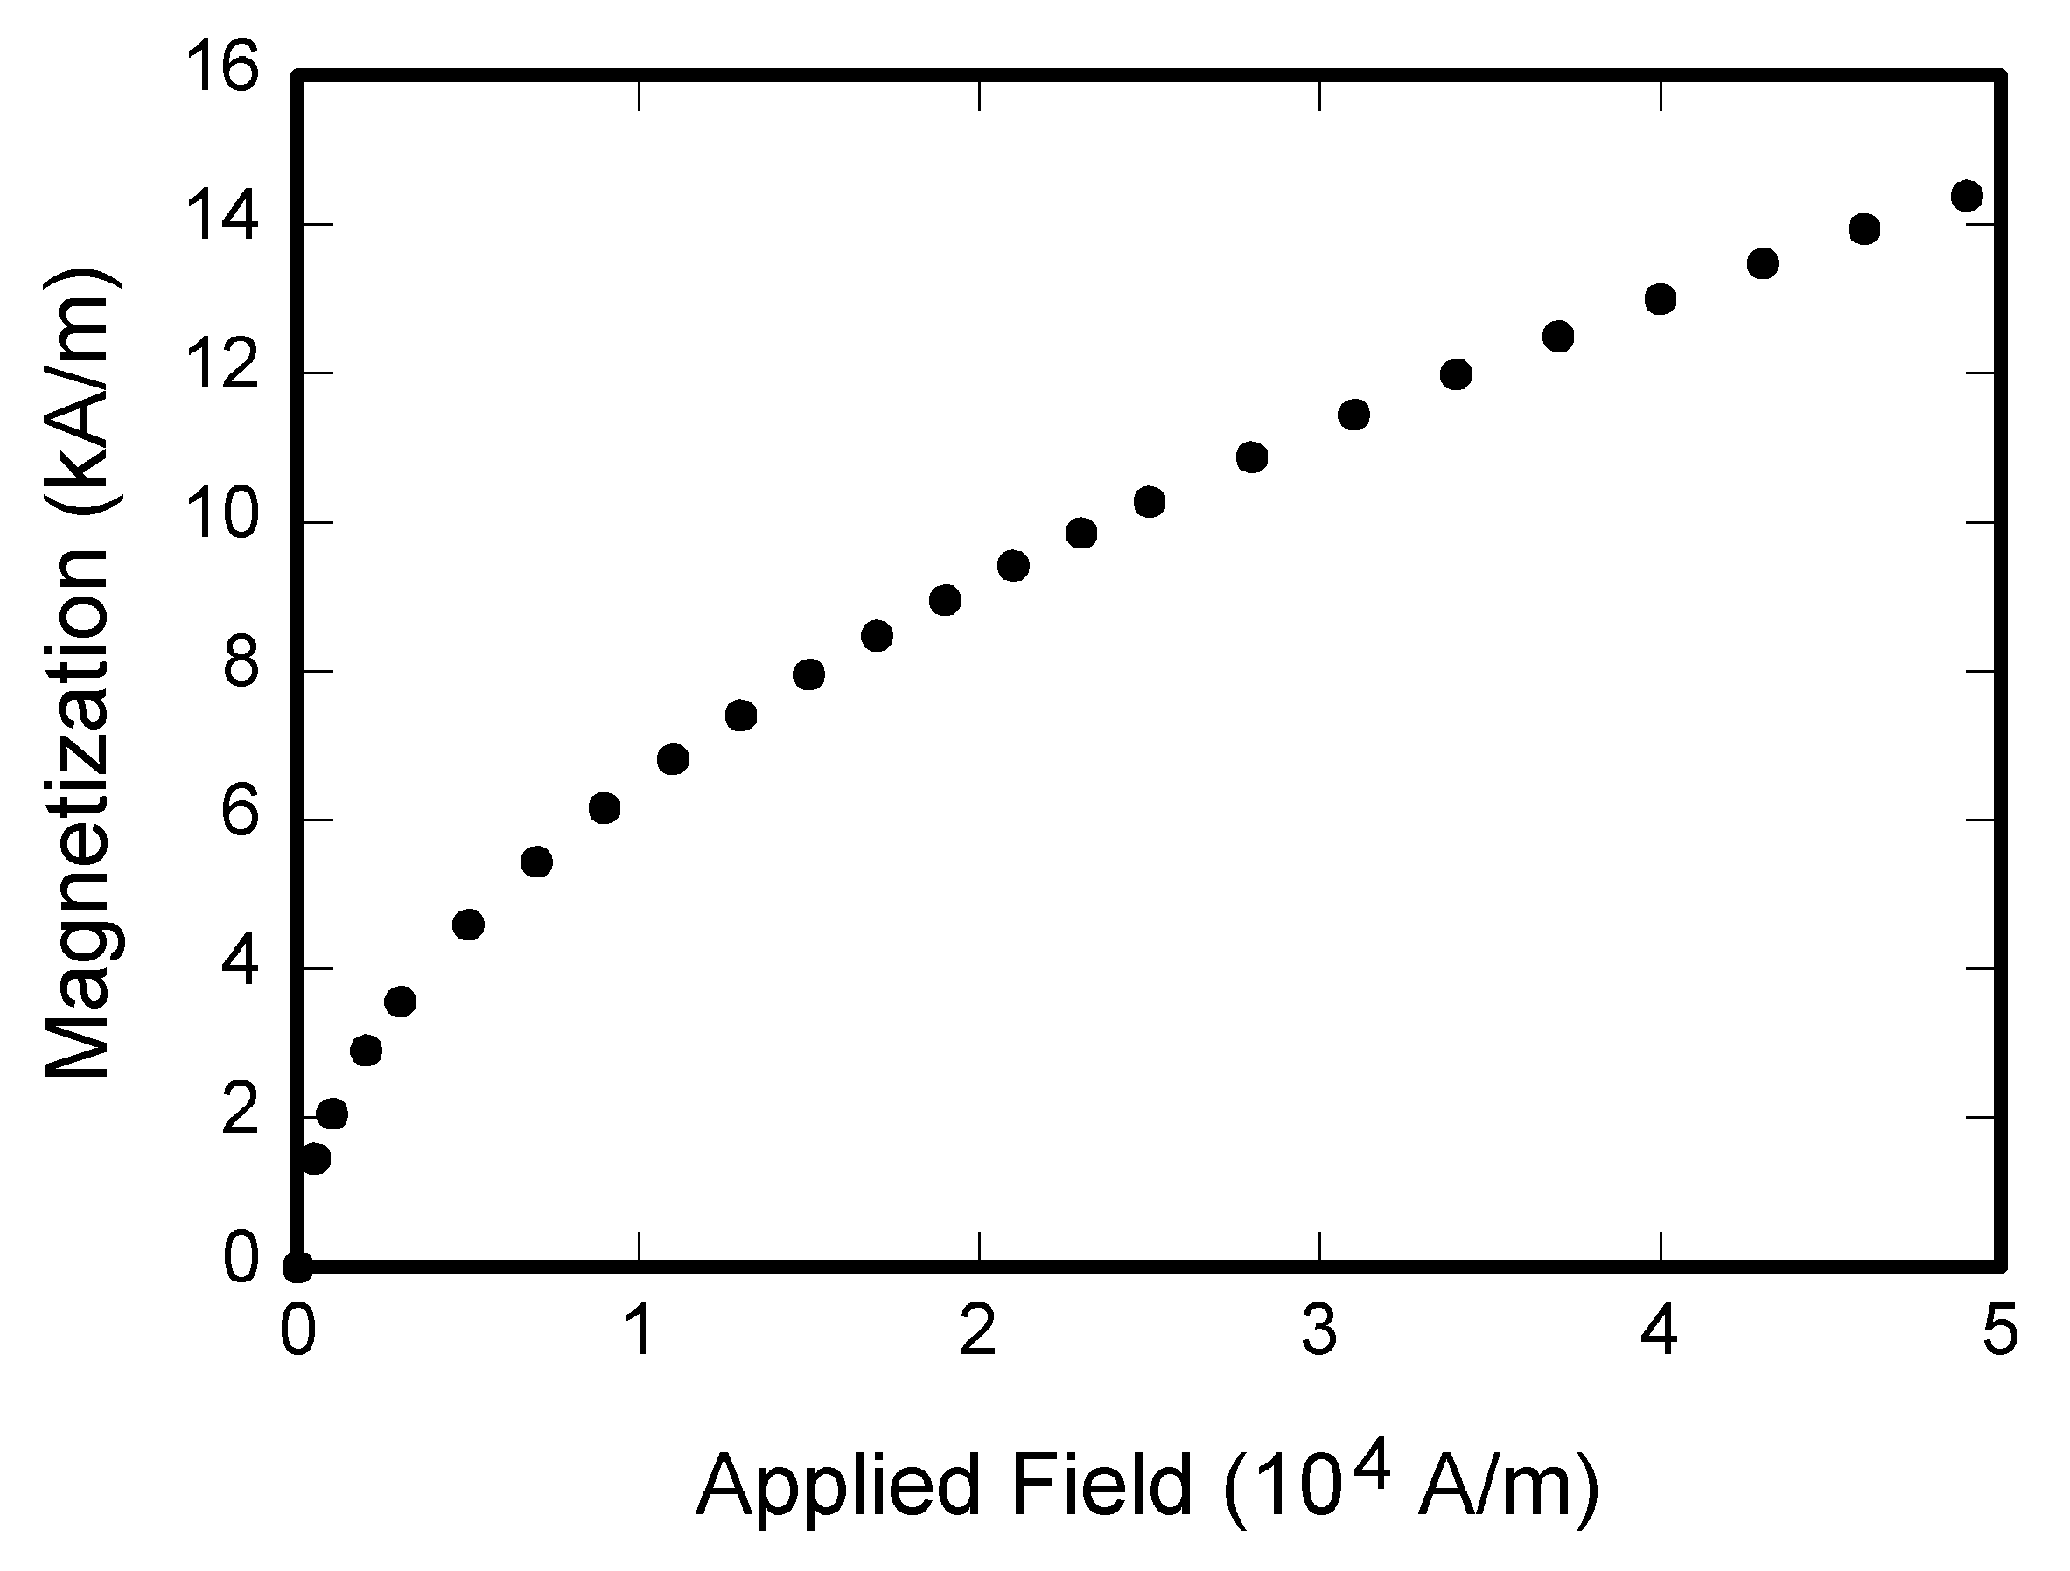
\includegraphics[width=1in,height=1.25in,clip,keepaspectratio]{fig1}}]{Michael Shell}
  Use $\backslash${\tt{begin\{IEEEbiography\}}} and then for the 1st argument use $\backslash${\tt{includegraphics}} to declare and link the author photo.
  Use the author name as the 3rd argument followed by the biography text.
\end{IEEEbiography}

\vspace{11pt}

\bf{If you will not include a photo:}\vspace{-33pt}
\begin{IEEEbiographynophoto}{John Doe}
  Use $\backslash${\tt{begin\{IEEEbiographynophoto\}}} and the author name as the argument followed by the biography text.
\end{IEEEbiographynophoto}

\vfill

\end{document}

